\chapter{\ac{lora} \ac{phy} Testing}

It has been repeatedly shown that \ac{lora} transmissions can be received at distances exceeding 10km in  unobstructed environments (free-space) when antennas are highly elevated \cite{3YP:LORA_RANGE_REVIEW}. However, these ideal radio conditions are unrealistic for swarm robots operating close to the ground in high-propagation environments such as forests. Therefore the first experiment in this paper identifies \ac{lora}'s physical performance and scenario specific limitations. 

\section{Methodology}
A full quantitive assessment was deemed infeasible given the sheer amount of data required to cover the full range of radio parameters and scenarios, coupled with this testing only being a project sub-goal. Therefore, a focus was taken to get enough data across a small selection of important scenarios and parameters, such that qualitative assessments could be made to aid protocol design. Due to the expected sparsity of robots, near field scenarios (when transmitter and receiver are very close) were of little interest; this left only the far field to test. For 868MHz signals this meant the distance between radios ($d_{tx}$) had to exceed 34.54cm (1 wavelength). 

 The two main transmission environments selected were free-space and in-forest; this was to give an understanding of both low-propagation and high-propagation scenarios. Data collection was mainly spread over two locations: \textbf{$L_{A}$} and \textbf{$L_{B}$} (split into \textbf{$L_{B1}$} and \textbf{$L_{B2}$}), identified in Figure \ref{fig:new_forest_map} and \ref{fig:stansted_map} respectively. All locations were rural and were therefore theoretically free from strong sources of external interference. Radio placement at each location was decided by first placing the transmitting radio (slave) at a fixed location, and then, using the furthest receivable point as the starting point for the receiving radio (master). From there the master was positioned closer towards the slave for each future test. In each scenario the main interest was ground level transmissions; however, to assess whether radio performance was actually compromised by the placement, comparative measurements were taken with an elevated antenna. 
 
  \begin{figure}[H]
    \centering
    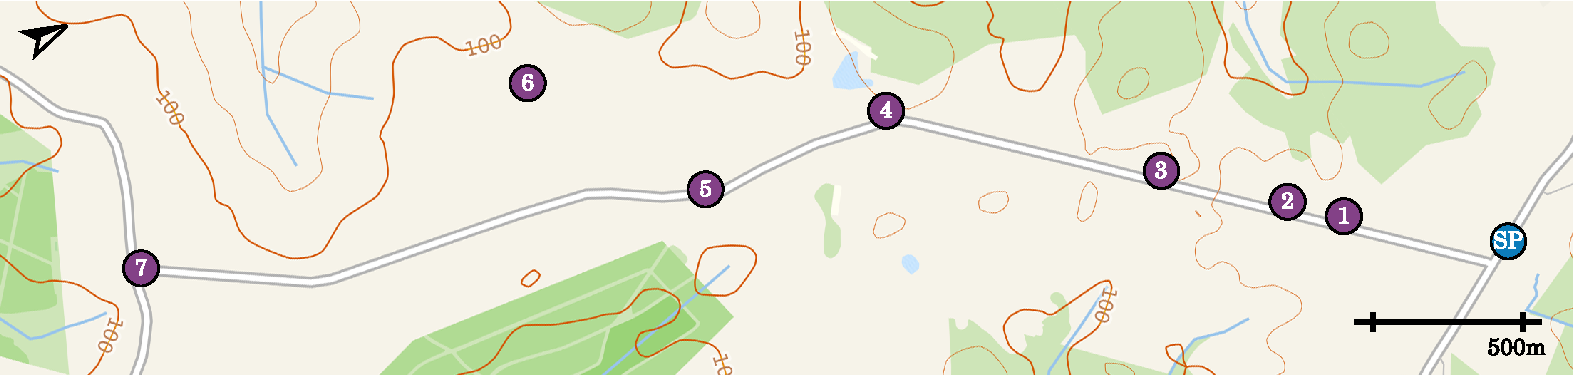
\includegraphics[width=\textwidth]{Figures/new_forest_light.pdf}
    \caption[Test Location: The New Forest, Hampshire, UK]{
    Test positions for \textbf{$L_A$} :  The New Forest, Hampshire, UK.\protect\footnotemark[1] \\
    \ac{sp} in open with \ac{los} to other points a combination of free-space and light vegetation. Positions and pictures in Appendix \ref{sec:new_forest_test_pos}. To the left of \ac{mp}7 vegetation density increases,  making \ac{mp}7 the furthest position viable for free-space testing.
    }
    \label{fig:new_forest_map}
\end{figure}

 In terms of radio parameters, \ac{sf} was the main focus due to it being an on option mostly unique to \ac{lora}; all values were tested for this in all locations (\ac{sf} = 7, 8, 9, 10, 11, 12). Variations using the lowest (4/5) and highest (4/8) \ac{cr}s were collected to verify \ac{fec} performance in an environment with little or no burst interference. Additionally, as the maximum transmission unit is often defined by the protocol, and the target was to inform the protocol, the effects of varying packet length were taken (\ac{pl} = 20, 128, 255). The rest of the parameters were fixed. The 868.1MHz \ac{cf} was used with \ac{tp} set to 14dBm so that the collected data would be relevant in regard to the \ac{etsi} regulations. The bandwidth was fixed to 125kHz so that radio sensitivity was only affected by the \ac{sf}. The programmed \ac{ps} was set to 8 to match that used by \ac{lorawan} \cite{3YP:LORAWAN_REGIONAL_PARAMS}. The number of packets (\ac{pc}) transmitted for each configuration was set to 50; though not guaranteed, this gives reasonable expectation of a normal distribution, thus allowing typical statistical analysis to be performed. See Table \ref{tab:TestDefinitions} for full test definitions.
 
 To test the point-to-point transmissions, two identical platforms, which together could log the performance of sending and receiving \ac{lora} transmissions, were required. The platforms had to be suitable for outdoor use, be able to test multiple radio configurations whilst on location and provide a mechanism to indicate to user when the maximum range had been reached. The hardware and corresponding software created for this purpose is detailed in Section \ref{sec:testing_platform}.
 \newpage
\vspace*{\fill}
\begingroup
 \begin{figure}[H]
    \centering
    \begin{tabular}{c}
    \subfloat[{
    Test positions for in-forest testing (\textbf{$L_{B1}$}). \ac{sp} in forest with \ac{los} to other points continually obstructed by a combination of leaved and bare trees. Positions and pictures in Appendix \ref{sec:stansted_forest_test_pos}. Large clump of \ac{mp}s where radio reception was inconsistent.
    }]
    {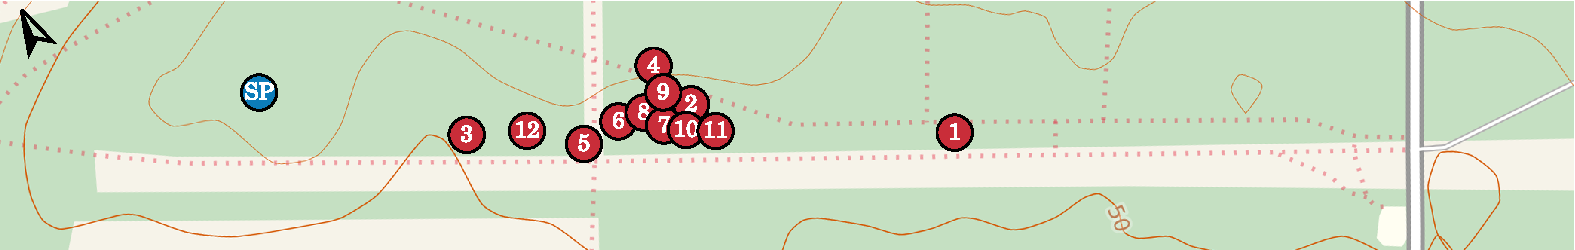
\includegraphics[width=\textwidth]{Figures/stansted_forest.pdf}\label{fig:stansted_map_forest}} 
    \\
    \subfloat[{
        Test positions for free-space testing (\textbf{$L_{B2}$}). \ac{sp} in open with \ac{los} completely free-space. Positions and pictures in Appendix \ref{sec:stansted_free_test_pos}. No access to right of \ac{mp}13.
    }]{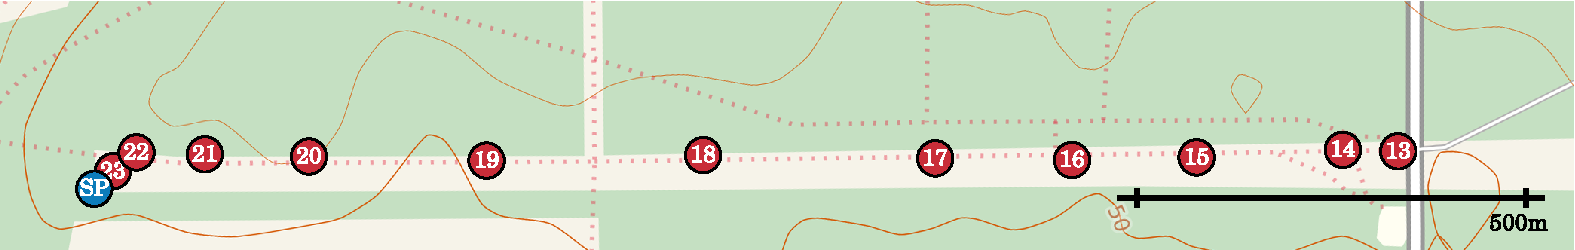
\includegraphics[width=\textwidth]{Figures/stansted_free_space.pdf}\label{fig:stansted_map_free}}
    \end{tabular}
    \caption[Test Location: Stansted Forest, West Sussex, UK]{
    Test locations for \textbf{$L_B$} :  Stansted Forest, West Sussex, UK.\footnotemark[1]
    }
    \label{fig:stansted_map}
\end{figure}


\begin{figure}[H]
    \centering
    \begin{tabular}{ccc}
    \subfloat[][$L_{A}$ : MP05 \\ (1.0m)]{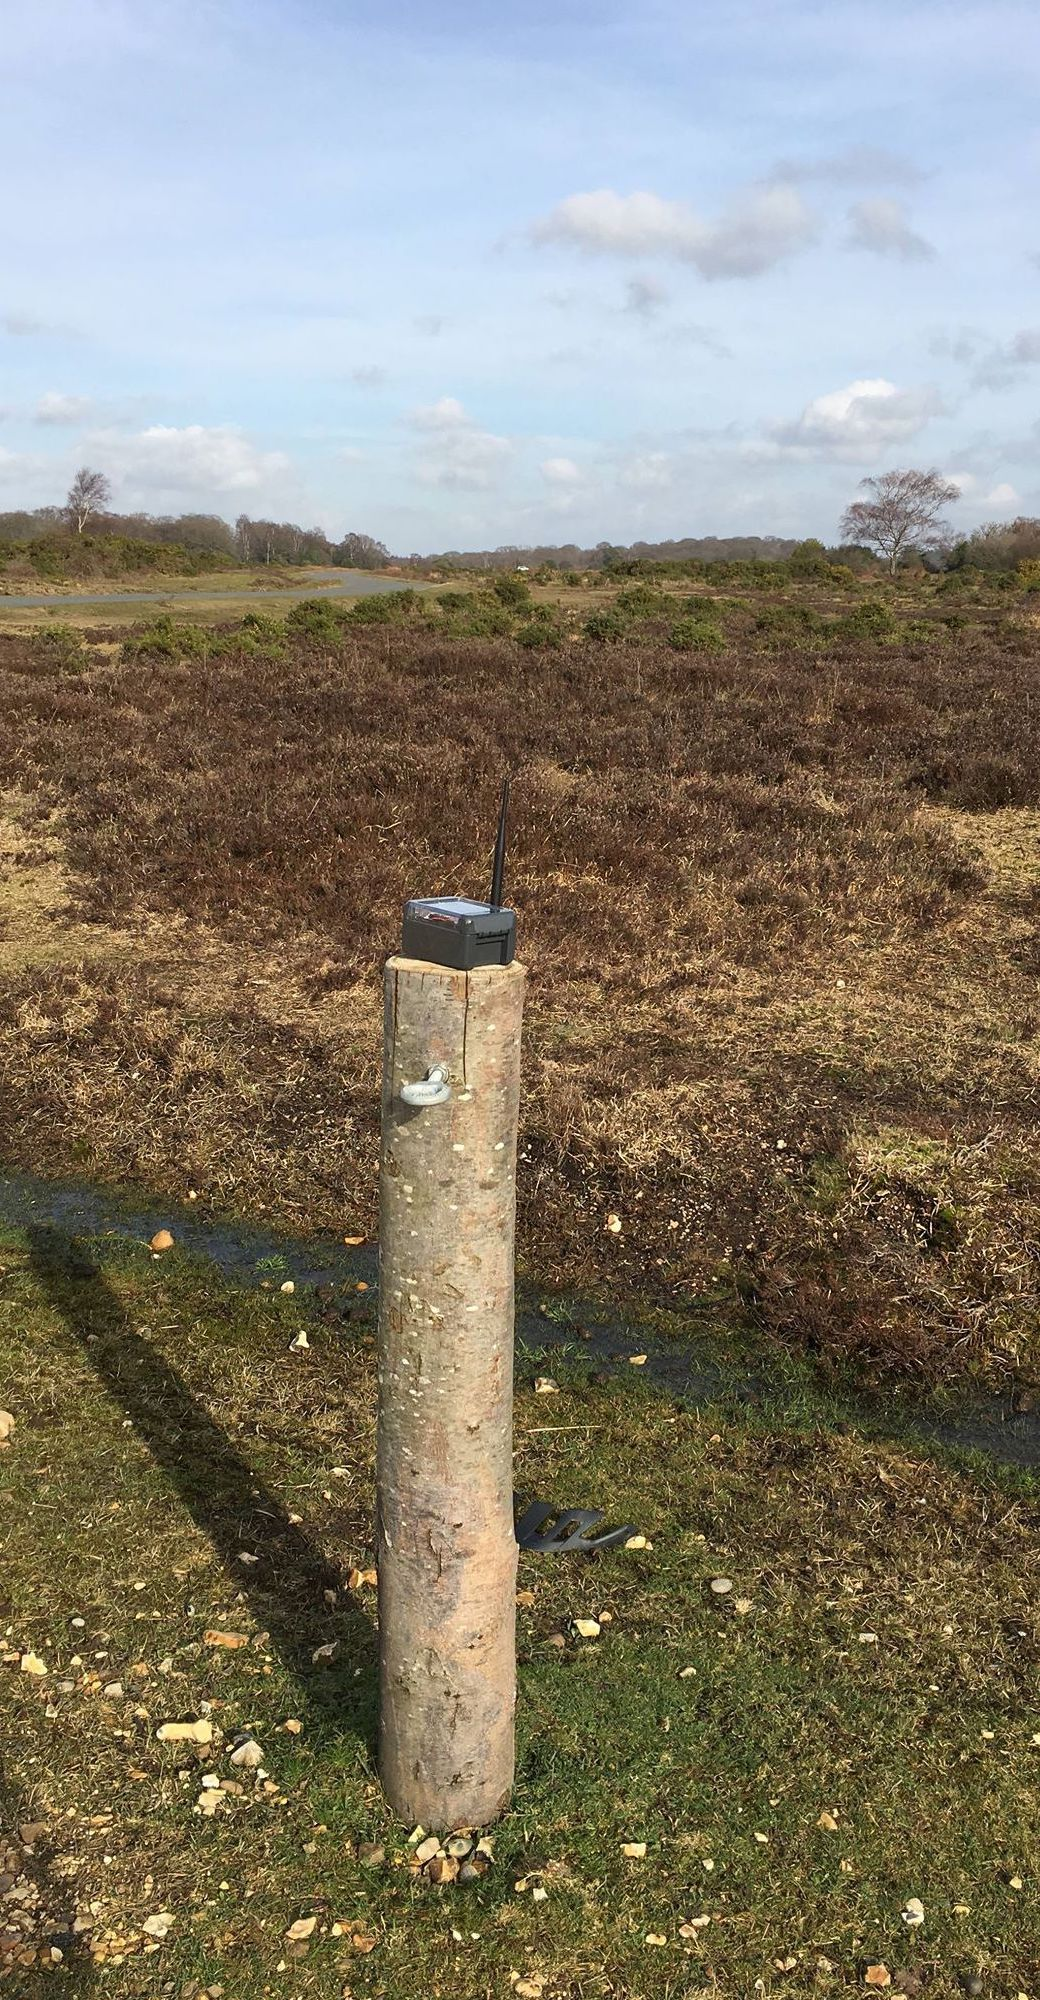
\includegraphics[height=7.5cm]{Figures/la_MP5_H1_0}}
    \hspace{2.5mm}
    \subfloat[][$L_{B1}$ : SP \\ (0.5m)]{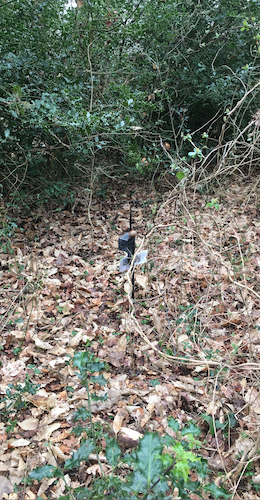
\includegraphics[height=7.5cm]{Figures/lb1_SP_H0_5}}
    \hspace{2.5mm}
    \subfloat[][$L_{B2}$ : MP16 \\ (0.0m)]{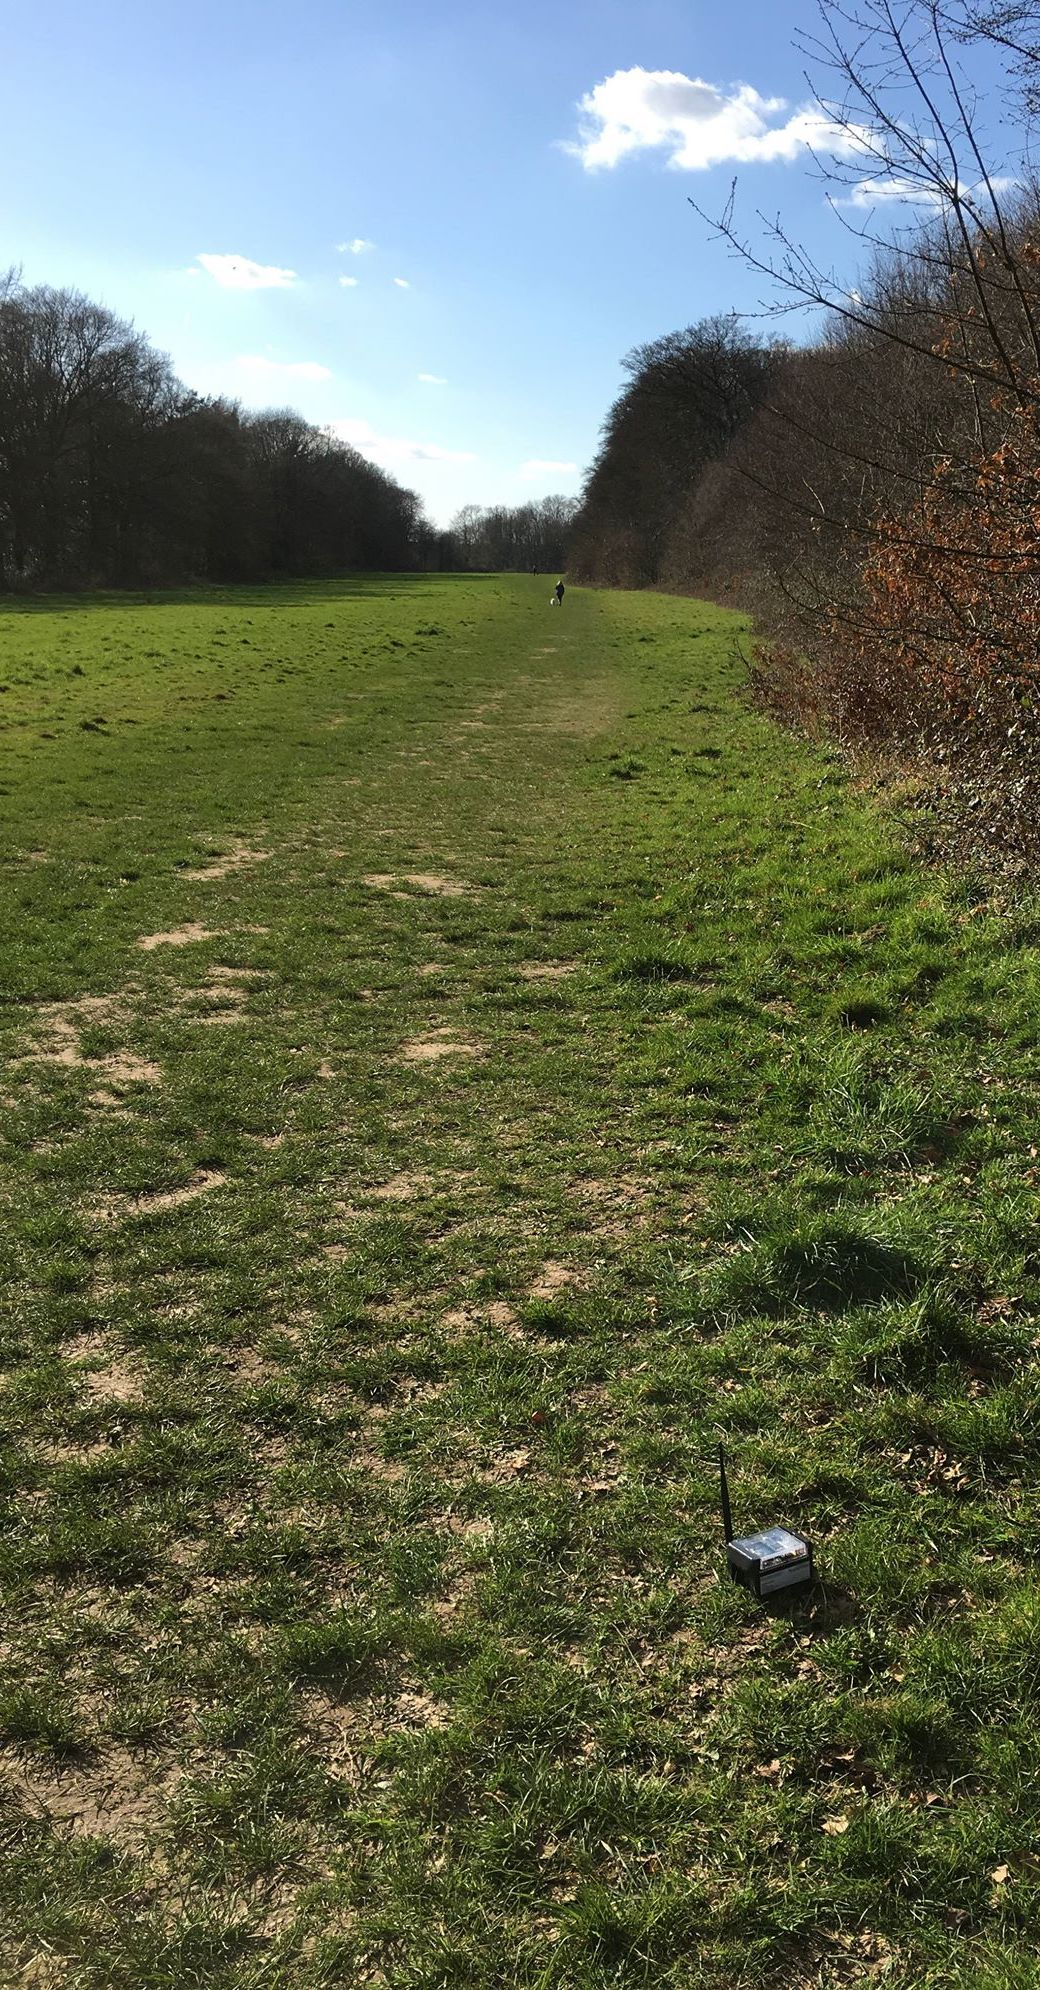
\includegraphics[height=7.5cm]{Figures/lb2_MP16_H0_0}}
    \end{tabular}
    \caption[Test location example]{Pictures of test environments and conditions. Although testing was split across multiple days at each location, the same dry conditions were present.}
    \label{fig:dataloggers}
\end{figure}
\endgroup
\vspace*{\fill}
\footnotetext[1]{
    	$\enskip $ Copyright © 2019 MapOSMatic/OCitySMap developers\\
    	\indent \indent $\enskip $ Map Data © 2019 OpenStreetMap contributors (see http://osm.org/copyright)\\
    	\indent \indent $\enskip $ British Style © MapQuest \\
    	\indent \indent $\enskip $ Contour Overlay © OpenSnowMap.org
}

 
\chapter{Testing  Platform}\label{sec:testing_platform}
\section{Hardware}
The basis of the designed test platform is HopeRF's\footnote{HopeRF Microelectronics Co. Ltd, China, https://www.hoperf.com/} RFM95W - a packet radio containing a \ac{lora} transceiver design licensed from Semtech; specifically, a broken out version from  Adafruit's\footnote{Adafruit, USA, https://www.adafruit.com/} is used. As a raw packet radio it provides direct access to the radio interface. An omni-directional 3dBi gain half-wavelength whip antenna is connected to the radio using a soldered uFL connector and a SMA to uFL connector. The net gain is assumed to be approximately 0dBm, after accounting for 1.5dBm loss in the cable (datasheet), 0.5dBm lost in the uFL connector (datasheet) and 1dBm lost through soldering (estimate). It is controlled by a Teensy\footnote{Teensy, https://www.pjrc.com/teensy/} 3.6 micro-controller, which also handles all logging responsibilities. A simple breakout circuit is implemented on strip-board to connect the components in a condensed package. Each breakout board features: a JST-PH2 battery connector, a coin cell holder for the Teensy's real-time-clock (\ac{rtc}), a power switch, a two-mode software switch, and three status LEDs. The schematic can be viewed in Figure \ref{fig:datalogger_schematic}. This is packaged to fit in an IP67 rated container with an internal lithium-polymer battery. Switches and SMA antenna connectors are external; these are IP67 rated and sealant is added where appropriate. The Teensy is equipped with an SD card for storage but, due to cost considerations, a GPS module is not implemented. A full breakdown of materials is listed in Figure \ref{fig:datalogger_cost}. The created test platforms, seen in Figure \ref{fig:dataloggers}, achieve the target of being a \ac{lora} datalogger suitable for all-weather.

\begin{figure}[H]
    \centering
    \begin{tabular}{cc}
    \subfloat[]{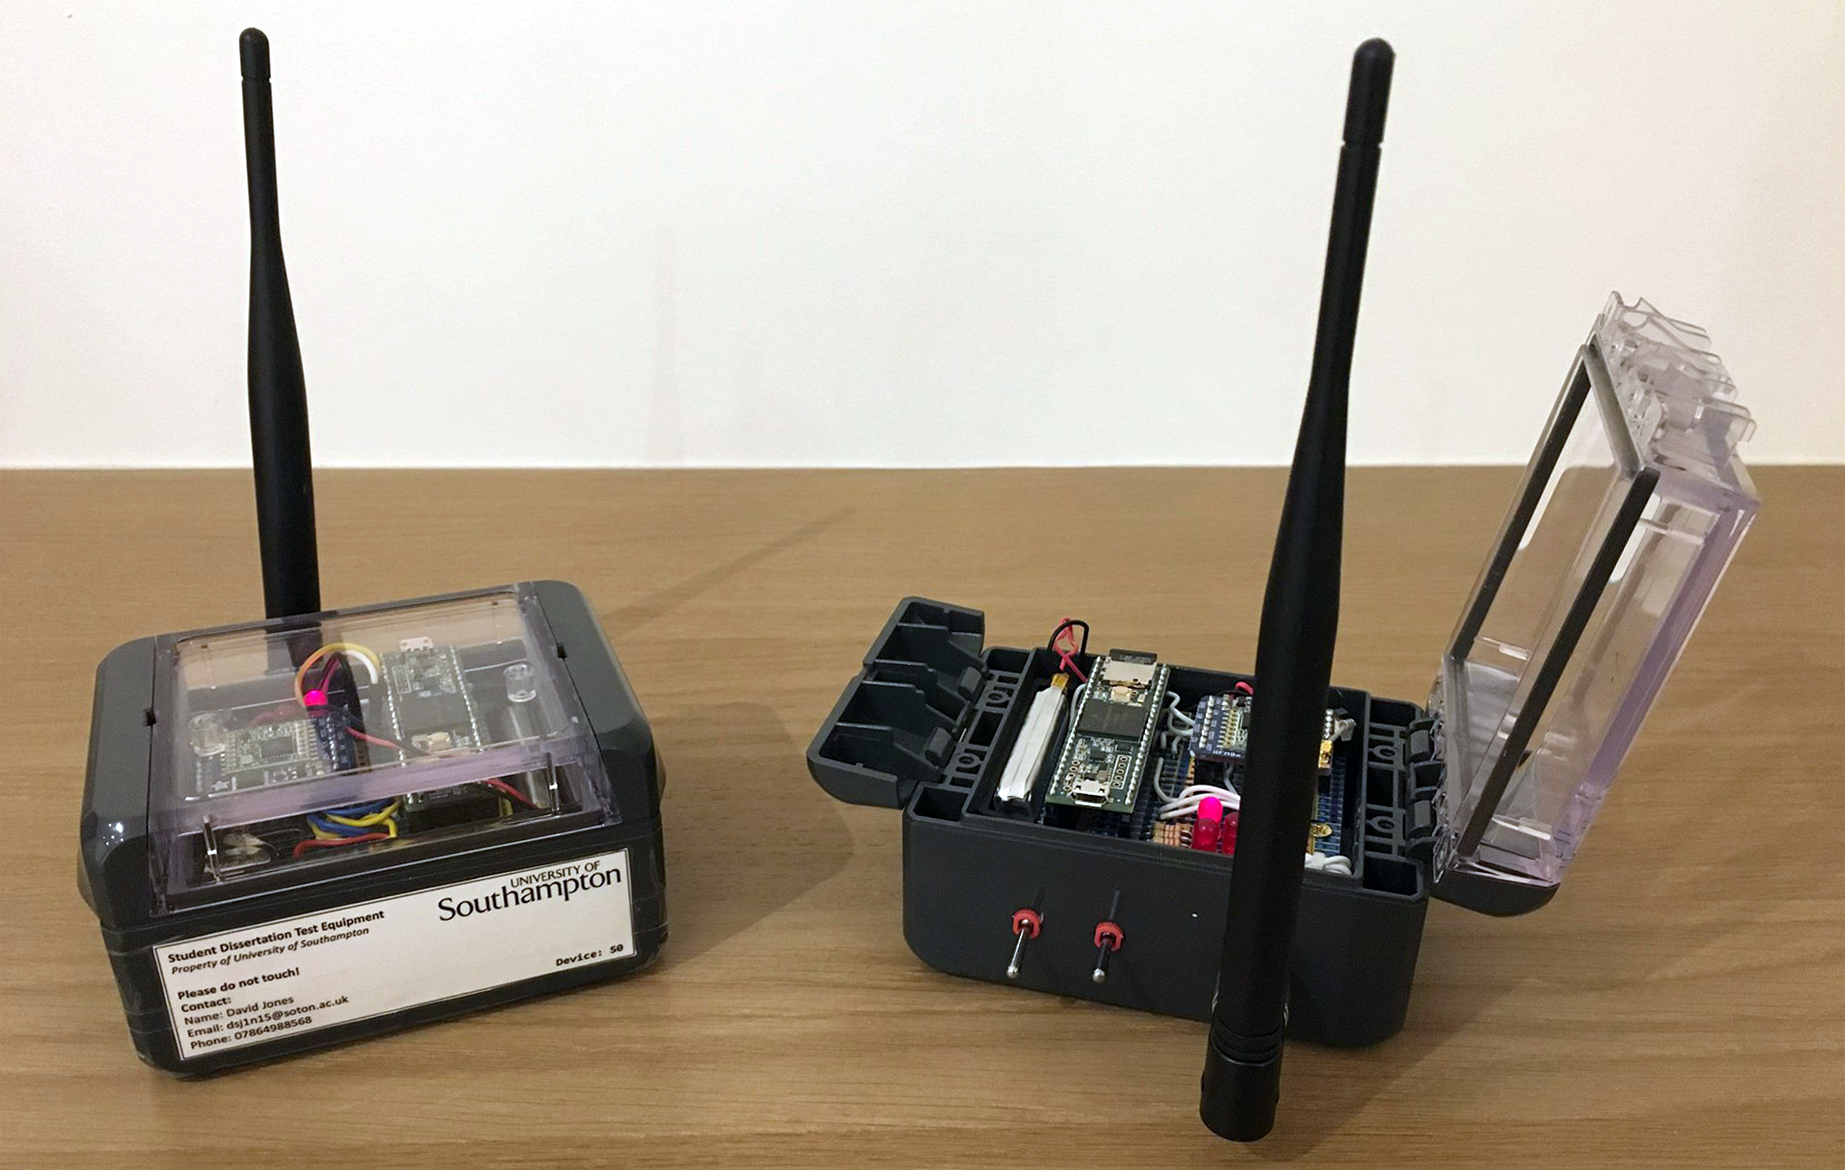
\includegraphics[height=5cm]{Figures/dl_both_devices.png}}
    \hspace{2.5mm}
    \subfloat[]{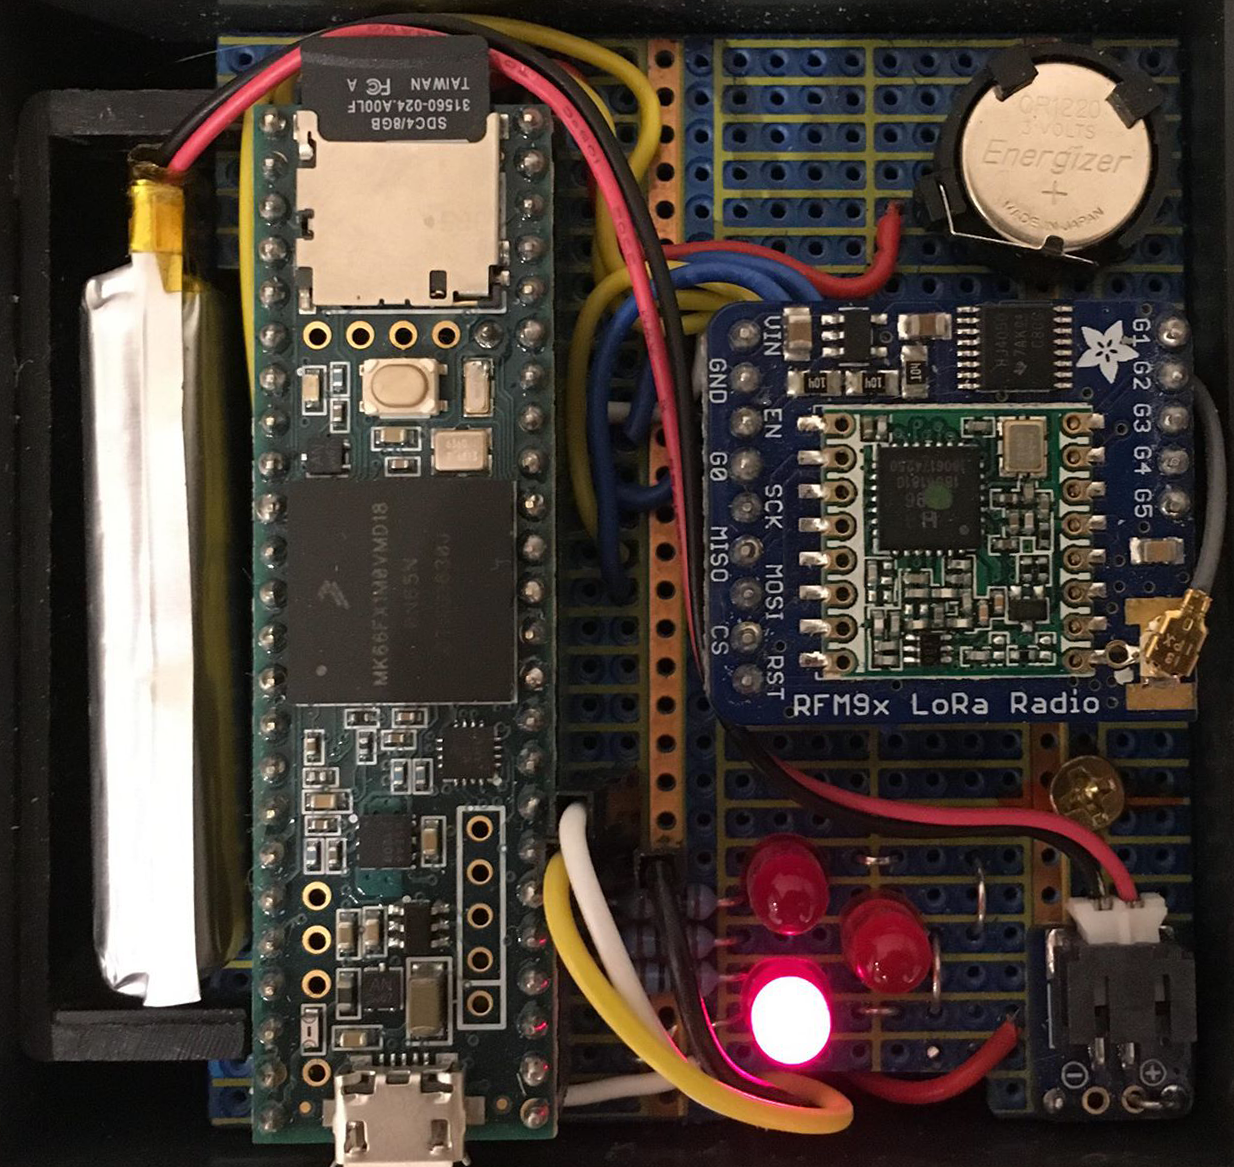
\includegraphics[height=5cm]{Figures/dl_circuit.png}}
    \end{tabular}
    \caption[Assembled testing platform]{External view of \texttt{S0} and \texttt{M0} platforms (left). Circuit view of \texttt{S0} (right); this is fixed into the assembly to avoid movement between tests. }
    \label{fig:dataloggers}
\end{figure}

\section{Software}\label{sec:test_platform_software}
The system is designed such that one device (a slave), can be left unattended at a fixed location and controlled by a second device (a master); this is achieved using a command control system, as explained in Figure \ref{fig:software_cmd_system}. Two command classes are defined for testing purposes; these are as follows:
\begin{itemize}
\vspace{-5mm}
	\item {\textbf{\texttt{HB\_CMD}}} : Command to trigger simple heartbeat functionality. When a slave receives this command it sends a heartbeat response (\textbf{\texttt{HB\_RSP}}) on the base configuration.
	\item {\textbf{\texttt{TD\_CMD}}} : Command to trigger execution of a test definition (\ac{td}). A \ac{td} holds a \ac{lora} configuration (values for \ac{cf}, \ac{sf}, \ac{tp}, \ac{bw}, \ac{cr}, \ac{pl}), a required \ac{pc}, and packet length. Figure \ref{fig:software_testdef_execution} explains the full control flow in detail.
	\end{itemize}
	
Slaves always listen to handle incoming commands, whereas the master can be set into two modes:
\vspace{-5mm}
\begin{itemize}
	\item \textbf{Heartbeat:} Sends periodic \texttt{HB\_CMD} commands, alerts user accordingly for every received or missed \textbf{\texttt{HB\_RSP}}.
	\item {\textbf{Run \ac{td}s:} Loads all stored \ac{td}s and handles them sequentially using \textbf{\texttt{TD\_CMD}}s.}
\end{itemize}
Interfacing with the radio is handled by the RH\_RF95 driver from the Radiohead\footnote{Radiohead, https://www.airspayce.com/mikem/arduino/RadioHead/} library. Operation of the software is detailed in Appendix \ref{sec:user_manual}.

\begin{figure}[p]
    \centering
    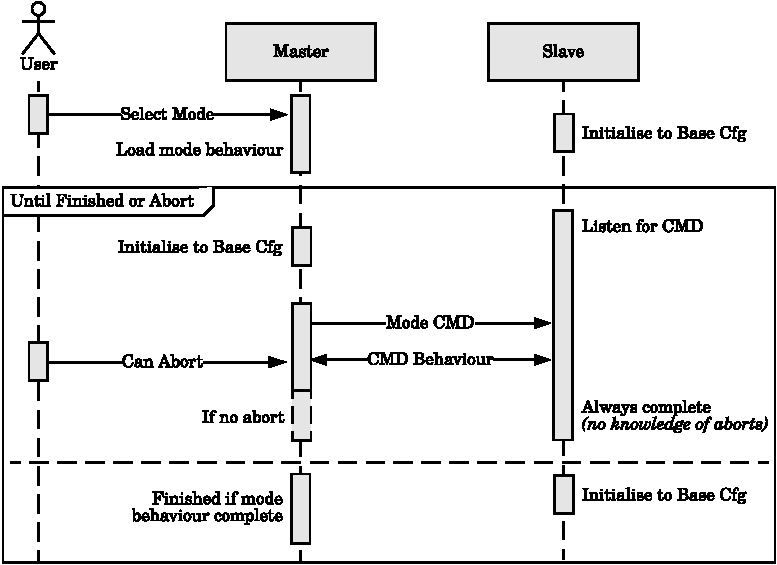
\includegraphics{Figures/software_cmd_system}
    \caption[Master-Slave command control method]{
    	Diagram showing master-slave command control method. Initially, both devices default to the same hardcoded radio parameters allowing two-way communication. This base state is chosen such that the expected range exceeds or matches that of the longest test range. When a mode is selected on the master, it sends the corresponding command to the listening slave and the behaviour is carried out. At any point the user may stop the master, and unless the slave is interacting with the master, it likely has no knowledge of this and will finish its behaviour. After command behaviour has finished the base configuration is reloaded in case it has been changed. In the case a master's mode requires multiple commands, the process repeats.
    }
    \label{fig:software_cmd_system}
\end{figure}
\begin{figure}[p]
    \centering
    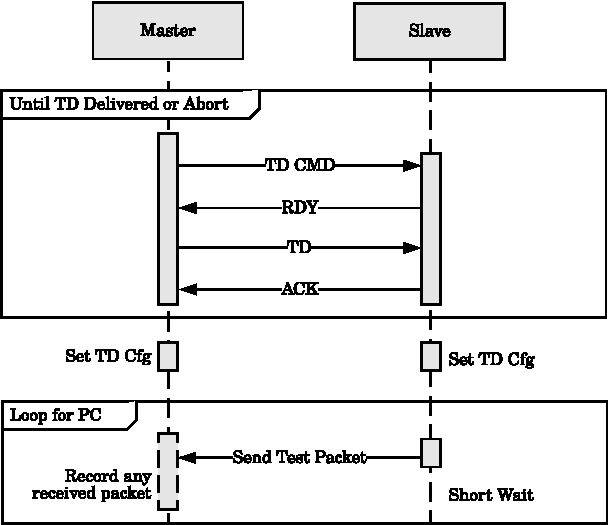
\includegraphics{Figures/software_testdef_execution}
    \caption[Master-Slave test definition execution method]{
    	Diagram showing execution of a single \ac{td}. After a \textbf{\texttt{TD\_CMD}} command is received, a short handshake takes place so that the master can share the \ac{td} to execute. After which both radios accordingly change their parameters and the slave sends the required \ac{pc}. Test packets are of length defined by the \ac{td} and contain a sequence identifier with the rest of data filled by a fixed data pattern. Any received packets are recorded along with \ac{rssi} and \ac{snr} values. Failed receives that occur due to bad CRCs are also recorded. This means that only transmissions where the preamble is not received are not recorded.
    }
    \label{fig:software_testdef_execution}
\end{figure}
\section{Results \& Discussion}
In total 498 test cases were executed, totalling 24,900 packet transmissions. Of this total, 19,545 were successfully received (78.5\%). The distribution of receive conditions for these individual points is indicated by Figure \ref{fig:density_plot}. When discussing results, received packets are considered alongside all other packets from the corresponding \ac{td}; allowing for packet receive percentage (\ac{prp}) and average \ac{snr}  metrics.

%Note that the raw \ac{rssi} values returned by the Radiohead library, and therefore the datalogger, are in fact packet strength for the SX1276 module; therefore a post-processing step must be applied to get separate packet strength and \ac{rssi} values valid for the RFM95W module.  Note that the logarithmic mean and standard deviation are used for decibel values.

\begin{figure}[H]
    \centering
   	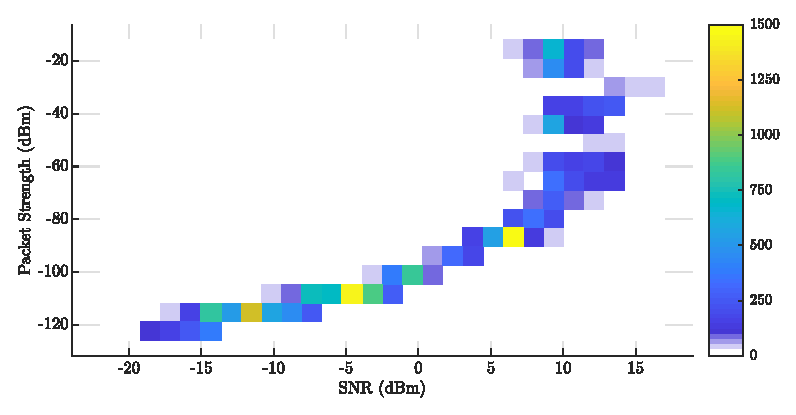
\includegraphics{Figures/density_plot}
    \caption[Test data distribution plot]{
    Density plot of received packet transmissions modelled as a bi-variate histogram with colour indicating received packet count. \\$Total\enskip Points = 19,545$
    }
    \label{fig:density_plot}
\end{figure}

Results are considered in two domains: the demodulation performance of the radio, and the environment effects. This is done because, even though actual receive performance varies with factors such as distance and attenuation, these can be abstracted into changes of the underlying \ac{snr} and \ac{rps} figures seen by the receiver. As there are no other transmission sources in this testing, theoretically, if these figures are within the required bounds for demodulation success, receives are successful.

\subsection{Demodulation Performance}\label{sec:demodulation_performance}
When $\text{\ac{snr}} \leq 0$ the \ac{rssi} value indicates the amount of noise seen by the receiver in the presence of no packet. When operating at 868MHz, the noise that the receiver should see is approximately the thermal noise floor ($-174+10 \log_{10}(\text{BW})$), plus the receiver noise figure; \ac{lora} implementations should have a noise figure of around 6dBm \cite{3YP:LORA_MOD_BASICS}. This indicates that for a 125kHz receive, the noise floor ($n_f$) should be -117dBm. The empirical noise floor calculated across all locations was -103dBm with a standard deviation of -109dBm; this is 14dBm ($24\times$) higher than expected. As the variance is low, this result indicates that the RFM95W hardware is of much poorer quality than expected, with a noise figure of 20dBm.

Whether the radio receives a transmission is dictated by whether the received power exceeds the receiver sensitivity ($R_S$). For \ac{lora} modules, $R_S = n_f - D_L$, where $D_L$ is the minimum SNR required for the current \ac{sf} (see Table \ref{tab:sf_effect}). This performance is explored in Figure \ref{fig:sf_pp_separate} and \ref{fig:sf_pp_fit}. In short, performance is close to theoretical for $\text{\ac{sf}} = 7, 8, 9, 10$ but $SF=11\enskip \& \enskip 12$ perform similarly to $\text{SF}=10$ with higher reliability. For all configurations, receive success is highly variant when approaching the empirical sensitivity.

\begin{figure}[H]
    \centering
   	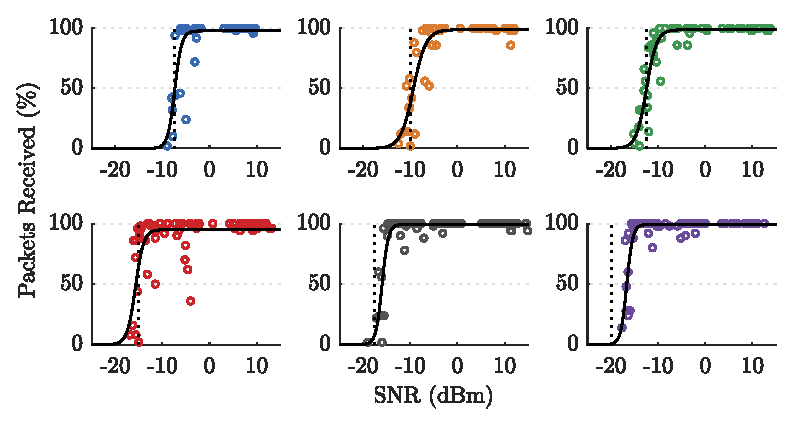
\includegraphics{Figures/sf_pp_separate_plot}
    \caption[Plots of \ac{snr} vs \ac{prp}]{
   \ac{td} mean \ac{snr} values plotted against their \ac{prp}s, separated by \ac{sf}s (Order = [[7, 8, 9], [10, 11, 12]]). For each \ac{sf} plot: $D_L$ is indicated by the dotted line and the solid line corresponds to the best-fit sigmoid function; these are repeated in Figure \ref{fig:sf_pp_fit}. Although the best-fits give a good representation of the general data pattern, and provide empirical demodulation cut-offs, they do not capture the high-variance receive behaviour when approaching the cut-off. This is reflected by: 62\%, 60\%, 66\%, 39\%, 77\% and 82\% of the respective training points fall inside the corresponding 95\% confidence interval.
    }
    \label{fig:sf_pp_separate}
\end{figure}

Theoretically, higher \ac{cr}s will result in more data being recovered from a transmissions allowing for greater receive success. Comparative tests are plotted in Figure \ref{fig:cr_pp_plot}. As no strong visual conclusions can be made, a null hypothesis is proposed; $H_{0} : $ \textit{The mean \ac{prp} does not increase between receives using \ac{cr} 4/5 and \ac{cr} 4/8} (otherwise written as $4/5_{\text{\ac{prp}}} \geq 4/8_{\text{\ac{prp}}}$). The respective means are 71.8\% and 72.5\%. Using a left-tailed Wilcoxon signed rank test for non-normal distributions gives $p=41.2\%$. With a 5\% significance level,  $H_{0}$ cannot be rejected, indicating that \ac{cr} has no effect on \ac{prp}.  Given that the \ac{snr}s are not significantly different \textit{(hypothesis testing omitted)} this indicates that receive drop-off and high variance when approaching sensitivity limits is the limiting factor for demodulation. The lack of \ac{cr} effect is unsurprising given that \ac{fec}'s main performance should be seen in the presence of burst interference.

\begin{figure}[H]
    \centering
   	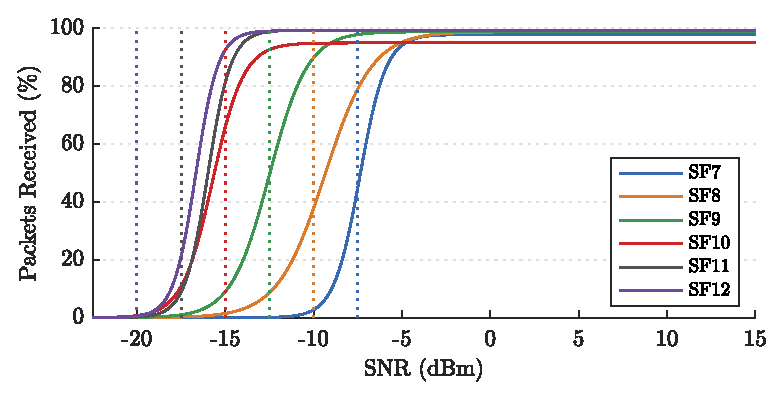
\includegraphics{Figures/sf_fit_plot}
    \caption[Sigmoid best-fits for \ac{snr} vs \ac{prp}]{
    Plot of sigmoid best-fits generated in Figure \ref{fig:sf_pp_separate}. The plot clearly demonstrates the positive effect increasing \ac{sf} has on demodulation performance of the receiver. For $\text{\ac{sf}}=7,8,9,10$ demodulation success starts dropping approximately 2.5dBm before $D_L$, with a 50\% \ac{prp} at $D_L$. This holds less so for \ac{sf}=11, for which drop-off starts around $D_L - 5dBm$, until $D_L$ where there is only a 10\% receive success. For \ac{sf}=12 drop-off starts around $D_L - 7.5dBm$, until $D_L$ where there is a 0\% receive success. Given the stable \ac{rssi} when $\text{\ac{snr}} < 0$, and that expected performance holds until a certain \ac{snr}, there is an indication that receiver sensitivity is not as high as stated.
     }
    \label{fig:sf_pp_fit}
\end{figure}

When the amount of data increases in a packet, its airtime will increase for the same configuration; this can lead to more channel noise being introduced (lower \ac{snr}) and receiver clock drift (lower demodulation performance). The effect this has on comparative tests is plotted in Figure \ref{fig:pl_pp_plot}. The mean \ac{prp}s of $\text{\ac{pl}} = 20, 128, 255$ are $81.7\%$, $78.8\%$ and $76.8\%$ respectively.  Three null hypotheses are proposed: $H^1_{0} : 20_{\text{\ac{prp}}} \leq 128_{\text{\ac{prp}}}$, $H^2_{0} : 20_{\text{\ac{prp}}} \leq 255_{\text{\ac{prp}}}$ and $H^3_{0} : 128_{\text{\ac{prp}}} \leq 255_{\text{\ac{prp}}}$. Using right-tailed Wilcoxon signed rank tests with 5\% significance, $H^1_{0}$ ($p=1.1\%$) and $H^2_{0}$ ($p=0.0\%$) are rejected but $H^3_{0}$ ($p=13.6\%$) is not. Therefore alternative hypotheses can be accepted  $H^1_{A}=20_{\text{\ac{prp}}} \geq 128_{\text{\ac{prp}}}$ and $H^2_{A}=20_{\text{\ac{prp}}} \geq 255_{\text{\ac{prp}}}$. Given that the \ac{snr}s are not significantly different, and that $H^3_{A}$ is narrowly rejected, a loose relationship between increased \ac{pl} and lower demodulation performance is assumed.
\begin{figure}[H]
    \centering
   	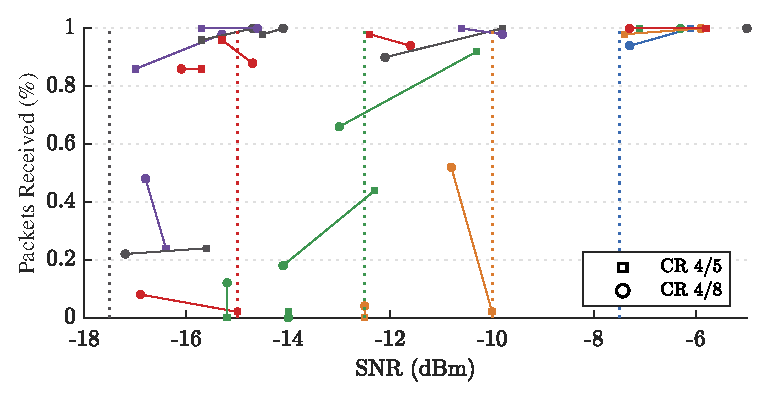
\includegraphics{Figures/cr_pp_plot}
    \caption[Effect of Coding Rate on \ac{snr} and \ac{prp}]{
    Plot of \ac{snr} and \ac{prp} for varying \ac{cr}s. Only configurations where all other factors are identical are included (e.g. height, location, \ac{lora} configuration). A line joins each set of points with a matching configuration. When $\text{SNR} > -5$, the \ac{prp} is nearly always 100\% and is therefore excluded.
    }
    \label{fig:cr_pp_plot}
\end{figure}

\begin{figure}[H]
    \centering
   	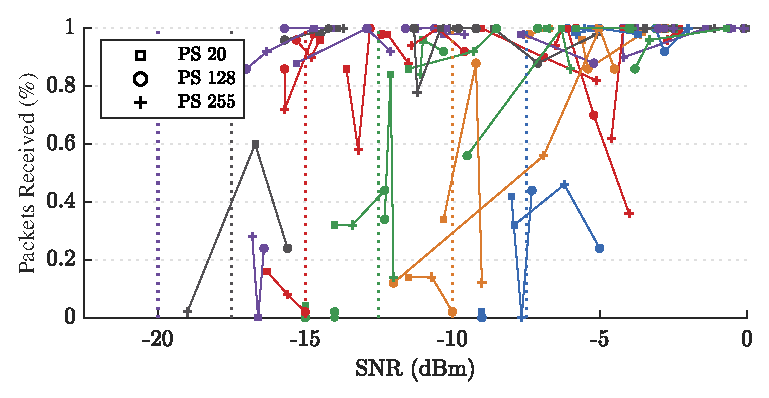
\includegraphics{Figures/pl_pp_plot}
    \caption[Effect of Packet Length on \ac{snr} and \ac{prp}]{
    Plot of \ac{snr} and \ac{prp} for varying \ac{pl}s. Only configurations where all other factors are identical are included. A line joins each set of points with a matching configuration. When $\text{SNR} > 0$, the \ac{prp} is nearly always 100\% and is therefore excluded.
    }
    \label{fig:pl_pp_plot}
\end{figure}

\subsection{Environment Effects}\label{sec:environment_propagation}
Free-space is the least attenuating environment possible and as such a transmission in free-space should represent the minimum path loss over a given distance; directly leading to the maximum transmission distance. The minimum free space path loss (\ac{fspl}), is calculated as $20\log_{10}(d) + 20\log_{10}(f) - 27.55$ where $d$ is distance in meters and $f$ is frequency in MHz \cite{3YP:ANTENNA_BOOK}. A more reasonable estimate must take into account effects such as ground reflection. The plain earth (\ac{pe}) model considers this and is calculated as $40\log_{10}(d) - 20\log_{10}(h_r) - 20\log_{10}(h_t)$ \cite{3YP:COMBINING_MODELS}. These are all plotted on Figure \ref{fig:distance_pl_plot}. Although transmissions occur at $0.0m$, receiver height ($h_r$) and transmitter height ($h_t$) are measured as the top of the antenna ($h_r = h_t = 0.17m$). As neither model fits the test data, with \ac{fspl} underestimating and \ac{pe} overestimating path loss, an empirical log-model is calculated as $91\log_{10}(d+362)-167$ (E-FSPL). This model fits the curve well but does not necessarily capture the variance caused by fading, as is reflected by only 83\% of data points falling in the 90\% confidence bound.

\begin{figure}[H]
    \centering
   	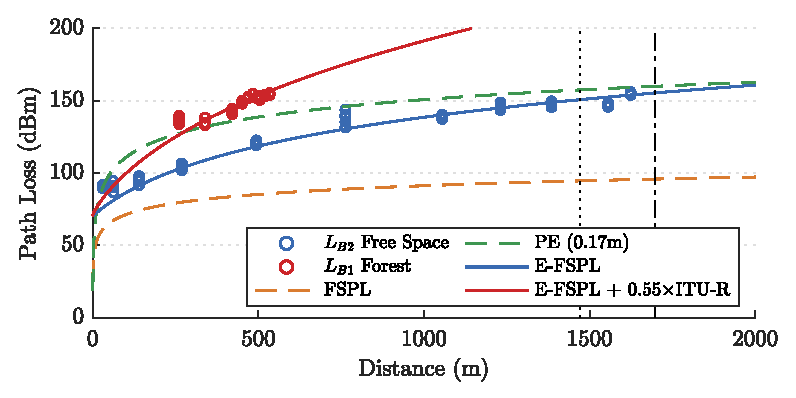
\includegraphics{Figures/distance_pl_plot}
    \caption[Effect of Distance on ground level Path Loss]{
    	Plot of path loss for ground level transmissions through free-space ($L_{B2}$) and forest environments ($L_{B1}$). The \ac{los} horizon and radio horizon are identified as the black dotted and dashed lines respectively.
    }
    \label{fig:distance_pl_plot}
\end{figure}
\vspace{-5mm}
Forests have high attenuation and should significantly increase path loss and reduce transmission distance. Due to the differences and complexity of vegetation, there is no de-facto propagation model, however, path loss should approximately match that of a vegetation model added to the environment's free space model \cite{3YP:COMBINING_MODELS}.  Many are explained in \cite{3YP:PROP_MODELS}, each of which can be made more flexible by applying an empirical multiplier, giving $L_{Total} = L_{FS} + \beta \times L_{Veg}$ \cite{3YP:EMPIRICAL_MULTIPLIER}. The in-forest model demonstrated is the free-space-fit model with the ITU-R vegetation model, where $\beta=0.55$. The model fits the in-forest test data; giving confidence in both the free-space fit model and that in-forest behaviour follows that of generalised \ac{rf} transmissions. Inter-transmission variance for a single test can be attributed to fading, however, it should be noted that test execution was inconsistent when approaching the transmission limit (480m+). This is likely a result of the bearing change between transmitter and receiver causing significant changes to the \ac{los} obstacles. To model this, either individual objects could be modelled or a varying empirical multiplier could be used. Although both the free-space and in-forest fit models serve the purpose of describing the test data, a full assessment of their generalisation would require significantly more data.

Transmissions at 868MHz are classed as ultra-high-frequency and usually have a maximum distance somewhere between the visual-horizon and radio-horizon \cite{3YP:ANTENNA_BOOK}. They are also susceptible to ground plane effects which can increase path loss. Varying radio heights for comparable measurements are plotted in Figure \ref{fig:height_pl_plot}. The decrease in path loss is clearly seen for both $0.0\text{m}\rightarrow 1.0\text{m} $ and $0.5\text{m}\rightarrow 1.0\text{m}$. The effect is less clear for $0.0\text{m}\rightarrow 0.5\text{m}$. In free-space with $d=10\text{m}$ on grass: path-loss for $0.0\text{m}$, $0.5\text{m}$ and $1.0\text{m}$ is 67dBm, 64dBm and 44dBm respectively. The increase between $0.0\text{m}$ and $0.5\text{m}$ is mathematically significant ($p=0.0$) but of an insignificant degree compared to $0.5\text{m}\rightarrow 1.0\text{m}$. These results are in-line with the principle that the ground effect is insignificant once antenna height is more than a few wavelengths \cite{3YP:ANTENNA_BOOK}. It is probable that transmissions are limited by the horizon in free-space given that the furthest receivable transmissions occur between the horizons for both $0.0\text{m}$ and $0.5\text{m}$ and there is sudden increase in path loss between the horizons for $0.0\text{m}$.

\begin{figure}[H]
    \centering
   	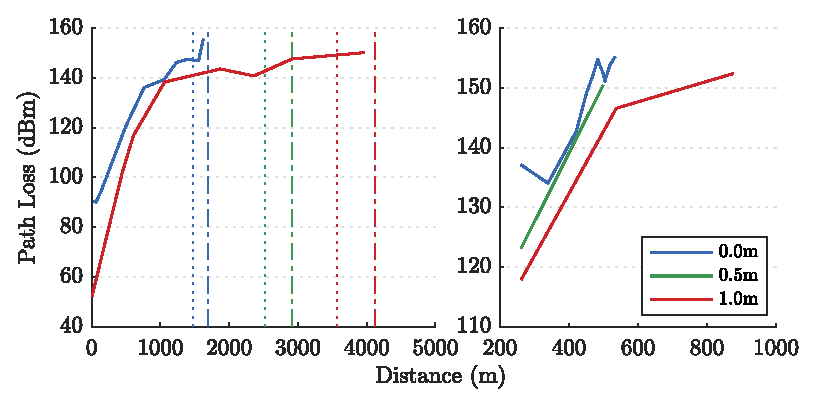
\includegraphics{Figures/height_pl_plot}
    \caption[Effect of Antenna Height on Path Loss]{
		Plot of path loss for varying heights in free-space (left) and in-forest (right). Path loss is the mean of all tests at location. The dotted lines identify the \ac{los} horizons. The dashed lines identify the radio horizons. Directly comparable data was not recorded for free-space 0.5m over multiple distances.
    }
    \label{fig:height_pl_plot}
\end{figure}

Overall range results indicate that \ac{lora} is suitable for single-hops in a system with sparsely separated radios; ranges of 500m can be expected for $\text{\ac{sf}}=11$ regardless of the propagation environment. However, even with the 1600m range offered in free space, single-hop point-to-point coverage to all radios is unlikely, leading to the expected dynamic mesh topology.




\subsection{Open (Free) Space}
High noise floor indicates that either the receiver's noise figure is not correct or there is more noise than expected in the environment. The fact that demodulation limit is nowhere near the true limit for SF10 onwards suggests that the cheaper radio does not perform correctly.


\section{Discussion}

\subsection{Forest}
\subsection{Radio Height}

% Testing platform
% Testing methodology 
% Distance in relatively open space (got)
% Distance in trees (got)
% Closeness to ground (got)
% Coding rate ??? (sort of got)
% Difference in slight movements (!!!)
%Lessons Learnt 
https://www.thethingsnetwork.org/forum/t/no-lower-rssi-than-121-dbm-possible-in-ttn/19890/15